\section{Web Semântica e Ontologia}

	Apesar de ser criada para possibilitar o acesso, intercâmbio e recuperação de informação de forma simples e rápida, o crescimento caótico e exponencial da \textit{Web} fez com que ela se tornasse um enorme repositório de documentos, dificultando o processo de recuperação dos mesmos \cite{Suarez2017}. Ainda hoje não existe nenhuma estratégia abrangente e satisfatória o suficiente para organizar documentos por meio de motores de busca que seja coerente com uma estrutura linguística \cite{Ci.Inf.1077}. Um outro exemplo de deficiência da \textit{Web} atual pode ser identificado em buscas feitas em sistemas de recuperação de informação, que usam palavras-chave nas buscas, considerando apenas o grau de similaridade e nível de ocorrência de certas palavras no documento, ou seja, a semântica da busca é desconsiderada \cite{Ci.Inf.1077}.
    
    Apresentada por \citeonline{10.2307/26059207}, a Web Semântica surge como uma proposta de estruturar os dados e informações disponíveis na \textit{Web}, para que agreguem significado e passem a ser computáveis por máquinas. A Web Semântica é definida por um conjunto de padrões definidos pela organização chamada \sigla{W3C}{World Wide Web Consortium}. Na sua proposta original, ela é definida como um extensão da \textit{Web} atual que tem como objetivo criar uma \textit{Web} universal dos conhecimentos da humanidade.
    
    Partindo dessa visão conceitual, \citeonline{10.2307/26059207} propuseram uma arquitetura de representação do conhecimento por camadas, conhecida pelos nomes de \textit{Semantic Web Stack}, \textit{Semantic Web Cake} e \textit{Semantic Web Layer Cake}, ilustrada na \autoref{fig:semanticcake}.
    
    \begin{figure}[htb]
    	\centering
        \caption{Arquitetura em camadas da Web Semântica.}
    	\label{fig:semanticcake}
        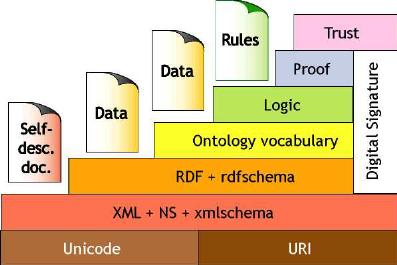
\includegraphics[width=0.7\linewidth]{images/semantic-web-cake}
        \fdireta{MIKA2005}
    \end{figure}
    
    A partir das bases \textit{Unicode} e \textit{URI}, a arquitura da Web Semântica se organiza nas seguintes camadas:
    
    \begin{itemize}
    	\item \textit{Unicode}: padrão de codificação de caracteres;
        \item \textit{URI}: permite a representação de um recurso por meio de uma cadeia de caracteres única;
        \item \sigla{XML}{\textit{eXtensible Markup Language}}: linguagem de marcação que permite a representação dos dados de forma sintática. Permite também a legibilidade das informações tanto por humanos quanto pelas máquinas;
        \item \sigla{RDF}{\textit{Resource Description Framework}}: modelo padrão para intercâmbio de dados. Possui mecanismos para suportar a integração de dados mesmo de esquemas distintos, além de suportar a evolução dos esquemas ao longo do tempo sem necessitar de mudanças nos consumidores de dados;
        \item \textit{Ontology}: estende a camada de descrição, fornecendo expressividade sobre conceitos, classificações, relações e inferências;
        \item \textit{Logic}: permite a definição de regras lógicas para deduzir e inferir novas informações. Essas regras são capazes de alterar dinamicamente a estrutura da ontologia;
        \item \textit{Proof}: provê mecanismos para averiguar a confiabilidade das fontes de informações;
        \item \textit{Trust}: representa o conhecimento validado e confiável;
        \textit{Digital Signature}: permite a integração de métodos de segurança que garantam a segurança da informação.
    \end{itemize}
    
    Uma importante contribuição da Web Semântica é a formalização da representação das ontologias.
    
    \subsection{Ontologias}
    
    	Ontologias da Web Semântica exercem um papel fundamental na confecção de um meio de descrição do conhecimento de especialistas de um domínio e, portanto, no \textit{design} de SADs baseados em conhecimento. Apesar do conceito de ontologia ser aplicável em vários campos, ele surgiu primeiro no ramo da filosofia, onde se refere ao estudo da realidade do ser,  da natureza e das suas relações \cite{sep-logic-ontology}.  Na área da ciência da computação, o conceito de ontologia é definido como uma especificação formal e explícita de conceitos relacionados em um determinado domínio de conhecimento \cite{Noy2001}. Mais especificamente, no campo da Web Semântica, \citeonline{9780123859662} definem ontologia como um esquema de representação que permite conceitualizar e estruturar um conhecimento de forma a habilitar a interpretação desse conhecimento pelas máquinas.
    
    	Como pode ser visto na \autoref{fig:kos-levels}, uma ontologia é o nível mais alto de um sistema de organização e representação do conhecimento, do inglês \sigla{KOS}{Knowledge Organization System}, que por sua vez é uma estrutura conceitual e computacional que permite representar conhecimentos de qualquer domínio por meio de entidades, classificações, relações semânticas e axiomas \cite{Cheng2016}. No nível mais baixo, os dados não possuem significado semântico, sendo dependentes do contexto da aplicação. O segundo nível envolve a definição de esquemas XML para alcançar a independência dos dados para com a aplicação, permitindo o intercâmbio de dados entre aplicações mas não entre domínios. Já no terceiro nível, os dados podem ser combinados a partir de diferentes domínios. No quarto e último nível, onde encontra-se as ontologias, é possível inferir novos dados a partir dos que já existem e compartilhá-los entre aplicações sem a necessidade de interferência humana \cite{9781439801567}.
        
        \begin{figure}[htbp]
        	\centering
        	\caption{Níveis de representação de dados na forma de conhecimento computável por máquinas.}
            \label{fig:kos-levels}
            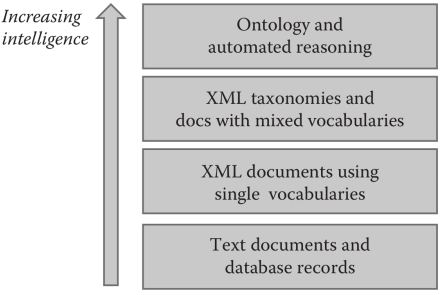
\includegraphics[width=0.7\linewidth]{images/kos-levels}
            \fdireta{9780123859662}
        \end{figure}
        
        Segundo \citeonline{Noy2001}, uma ontologia é especificada pelos seguintes componentes:
        
        \begin{itemize}
        	\item Classes: descrevem os conceitos de um domínio, habilitando a classificação e organização dos indivíduos em um sistema lógico e hierárquico;
            \item Indivíduos: são as instâncias das classes, utilizados para representar elementos específicos, os objetos de interesse do domínio;
            \item Relações: representam as interações entre os conceitos de um domínio e as propriedades presentes nas classes e indivíduos, podendo ter características próprias; 
            \item Axiomas: modelam as regras assumidas como verdadeiras no domínio considerado, sendo possível associar relacionamentos entre indivíduos além de fornecer características descritivas e lógicas para as classes.
        \end{itemize}
        
        A partir dessas definições, existem padrões adotados pela comunidade para implementar os conceitos da Web Semântica. RDF e OWL são alguns dos padrões recomendados pela W3C e que serão apresentados a seguir.
        
	\subsection{\textit{Resource Description Framework} e \textit{Web Ontology Language}}
    
    	RDF é um modelo padrão para intercâmbio de dados para que estes sejam compartilhados e reusados por meio das fronteiras das aplicações, empresas e comunidades. O RDF é usado em diferentes domínios de aplicação como \textit{resource discovery} com o objetivo de aprimorar as capacidades dos motores de busca, catalogação de documentos, descrição de conteúdo e suas relações e descrição de propriedade intelectual. Seu modelo consiste em um conjunto de três tipos de objetos, chamados de tripla RDF. Os componentes são:
        
        \begin{itemize}
        	\item Sujeito: representa os recursos e são identificados por meios de URIs;
            \item Predicado:representa os aspectos, características, atributos ou relações específicas que descrevem o sujeito, onde cada predicado possui um valor específico e relaciona um sujeito a um objeto;
            \item Objeto: um valor de uma propriedade ou um recurso específico que representa uma característica do sujeito.
        \end{itemize}
        
        Com triplas RDF é possível explicitar relações entre dois objetos, mas não é possível fazer modelagens mais expressivas nem mesmo inferências. Para alcançar essas características é necessário que a ontologia seja descrita em OWL.
        
        OWL é uma linguagem recomendada pela W3C para representação e compartilhamento de ontologias na \textit{Web}. Ela foi projetada para aplicações que necessitam processar a informação ao invés de apenas organizá-las em nós \cite{Mcguinness2004}. OWL permite que a semântica seja explicitamente associada ao conteúdo dos dados na \textit{web} e formalmente especificada por meio de ontologias compartilhadas na \textit{internet}.
        
        \begin{figure}[htbp]
        	\centering
            \caption{Diagrama de Venn sobre o relacionamento estre os perfis da linguagem OWL2.}
            \label{fig:owl2-profiles}
            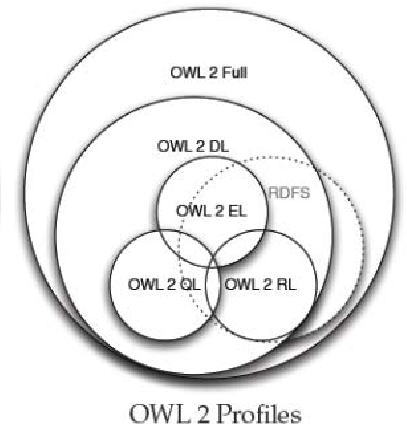
\includegraphics[width=0.7\linewidth]{images/owl2-profiles}
            \fadaptada{Alamri_2012}
        \end{figure}
        
        A versão mais recente desta linguagem é a OWL2 que possui cinco diferentes perfis (sub-linguagens), como pode ser visto na \autoref{fig:owl2-profiles}. Cada um desses perfis permite um nível diferente de expressividade para cada cenário de aplicação. Esses perfis são:
        
        \begin{itemize}
        	\item Full: permite a máxima expressividade e liberdade sintática mas sem garantia computacional;
            \item DL: desenvolvido para aplicações que requerem a máxima expressividade enquanto mantém a decidibilidade (computações terminam em tempo finito) e computabilidade (conclusões são garantidas de serem computáveis). Nesse perfil existem limitações sobre os recursos da linguagem para garantir as duas características citadas anteriormente;
            \item EL: baseado em lógica descritiva, é útil para aplicações que contém um grande número de propriedades e/ou classes;
            \item QL: permite o processo de raciocínio, do inglês \textit{reasoning}, eficiente para grandes quantidades de dados estruturados em ontologias relativamente simples;
            \item RL: direcionado para aplicações que exigem \textit{reasoning} escalável em troca de restrições na expressividade. Favorece a implementação utilizando tecnologias baseadas em regras.
        \end{itemize}